% Options for packages loaded elsewhere
\PassOptionsToPackage{unicode}{hyperref}
\PassOptionsToPackage{hyphens}{url}
\PassOptionsToPackage{dvipsnames,svgnames,x11names}{xcolor}
%
\documentclass[
  letterpaper,
  DIV=11,
  numbers=noendperiod]{scrartcl}

\usepackage{amsmath,amssymb}
\usepackage{iftex}
\ifPDFTeX
  \usepackage[T1]{fontenc}
  \usepackage[utf8]{inputenc}
  \usepackage{textcomp} % provide euro and other symbols
\else % if luatex or xetex
  \usepackage{unicode-math}
  \defaultfontfeatures{Scale=MatchLowercase}
  \defaultfontfeatures[\rmfamily]{Ligatures=TeX,Scale=1}
\fi
\usepackage{lmodern}
\ifPDFTeX\else  
    % xetex/luatex font selection
\fi
% Use upquote if available, for straight quotes in verbatim environments
\IfFileExists{upquote.sty}{\usepackage{upquote}}{}
\IfFileExists{microtype.sty}{% use microtype if available
  \usepackage[]{microtype}
  \UseMicrotypeSet[protrusion]{basicmath} % disable protrusion for tt fonts
}{}
\makeatletter
\@ifundefined{KOMAClassName}{% if non-KOMA class
  \IfFileExists{parskip.sty}{%
    \usepackage{parskip}
  }{% else
    \setlength{\parindent}{0pt}
    \setlength{\parskip}{6pt plus 2pt minus 1pt}}
}{% if KOMA class
  \KOMAoptions{parskip=half}}
\makeatother
\usepackage{xcolor}
\setlength{\emergencystretch}{3em} % prevent overfull lines
\setcounter{secnumdepth}{-\maxdimen} % remove section numbering
% Make \paragraph and \subparagraph free-standing
\ifx\paragraph\undefined\else
  \let\oldparagraph\paragraph
  \renewcommand{\paragraph}[1]{\oldparagraph{#1}\mbox{}}
\fi
\ifx\subparagraph\undefined\else
  \let\oldsubparagraph\subparagraph
  \renewcommand{\subparagraph}[1]{\oldsubparagraph{#1}\mbox{}}
\fi

\usepackage{color}
\usepackage{fancyvrb}
\newcommand{\VerbBar}{|}
\newcommand{\VERB}{\Verb[commandchars=\\\{\}]}
\DefineVerbatimEnvironment{Highlighting}{Verbatim}{commandchars=\\\{\}}
% Add ',fontsize=\small' for more characters per line
\usepackage{framed}
\definecolor{shadecolor}{RGB}{241,243,245}
\newenvironment{Shaded}{\begin{snugshade}}{\end{snugshade}}
\newcommand{\AlertTok}[1]{\textcolor[rgb]{0.68,0.00,0.00}{#1}}
\newcommand{\AnnotationTok}[1]{\textcolor[rgb]{0.37,0.37,0.37}{#1}}
\newcommand{\AttributeTok}[1]{\textcolor[rgb]{0.40,0.45,0.13}{#1}}
\newcommand{\BaseNTok}[1]{\textcolor[rgb]{0.68,0.00,0.00}{#1}}
\newcommand{\BuiltInTok}[1]{\textcolor[rgb]{0.00,0.23,0.31}{#1}}
\newcommand{\CharTok}[1]{\textcolor[rgb]{0.13,0.47,0.30}{#1}}
\newcommand{\CommentTok}[1]{\textcolor[rgb]{0.37,0.37,0.37}{#1}}
\newcommand{\CommentVarTok}[1]{\textcolor[rgb]{0.37,0.37,0.37}{\textit{#1}}}
\newcommand{\ConstantTok}[1]{\textcolor[rgb]{0.56,0.35,0.01}{#1}}
\newcommand{\ControlFlowTok}[1]{\textcolor[rgb]{0.00,0.23,0.31}{#1}}
\newcommand{\DataTypeTok}[1]{\textcolor[rgb]{0.68,0.00,0.00}{#1}}
\newcommand{\DecValTok}[1]{\textcolor[rgb]{0.68,0.00,0.00}{#1}}
\newcommand{\DocumentationTok}[1]{\textcolor[rgb]{0.37,0.37,0.37}{\textit{#1}}}
\newcommand{\ErrorTok}[1]{\textcolor[rgb]{0.68,0.00,0.00}{#1}}
\newcommand{\ExtensionTok}[1]{\textcolor[rgb]{0.00,0.23,0.31}{#1}}
\newcommand{\FloatTok}[1]{\textcolor[rgb]{0.68,0.00,0.00}{#1}}
\newcommand{\FunctionTok}[1]{\textcolor[rgb]{0.28,0.35,0.67}{#1}}
\newcommand{\ImportTok}[1]{\textcolor[rgb]{0.00,0.46,0.62}{#1}}
\newcommand{\InformationTok}[1]{\textcolor[rgb]{0.37,0.37,0.37}{#1}}
\newcommand{\KeywordTok}[1]{\textcolor[rgb]{0.00,0.23,0.31}{#1}}
\newcommand{\NormalTok}[1]{\textcolor[rgb]{0.00,0.23,0.31}{#1}}
\newcommand{\OperatorTok}[1]{\textcolor[rgb]{0.37,0.37,0.37}{#1}}
\newcommand{\OtherTok}[1]{\textcolor[rgb]{0.00,0.23,0.31}{#1}}
\newcommand{\PreprocessorTok}[1]{\textcolor[rgb]{0.68,0.00,0.00}{#1}}
\newcommand{\RegionMarkerTok}[1]{\textcolor[rgb]{0.00,0.23,0.31}{#1}}
\newcommand{\SpecialCharTok}[1]{\textcolor[rgb]{0.37,0.37,0.37}{#1}}
\newcommand{\SpecialStringTok}[1]{\textcolor[rgb]{0.13,0.47,0.30}{#1}}
\newcommand{\StringTok}[1]{\textcolor[rgb]{0.13,0.47,0.30}{#1}}
\newcommand{\VariableTok}[1]{\textcolor[rgb]{0.07,0.07,0.07}{#1}}
\newcommand{\VerbatimStringTok}[1]{\textcolor[rgb]{0.13,0.47,0.30}{#1}}
\newcommand{\WarningTok}[1]{\textcolor[rgb]{0.37,0.37,0.37}{\textit{#1}}}

\providecommand{\tightlist}{%
  \setlength{\itemsep}{0pt}\setlength{\parskip}{0pt}}\usepackage{longtable,booktabs,array}
\usepackage{calc} % for calculating minipage widths
% Correct order of tables after \paragraph or \subparagraph
\usepackage{etoolbox}
\makeatletter
\patchcmd\longtable{\par}{\if@noskipsec\mbox{}\fi\par}{}{}
\makeatother
% Allow footnotes in longtable head/foot
\IfFileExists{footnotehyper.sty}{\usepackage{footnotehyper}}{\usepackage{footnote}}
\makesavenoteenv{longtable}
\usepackage{graphicx}
\makeatletter
\def\maxwidth{\ifdim\Gin@nat@width>\linewidth\linewidth\else\Gin@nat@width\fi}
\def\maxheight{\ifdim\Gin@nat@height>\textheight\textheight\else\Gin@nat@height\fi}
\makeatother
% Scale images if necessary, so that they will not overflow the page
% margins by default, and it is still possible to overwrite the defaults
% using explicit options in \includegraphics[width, height, ...]{}
\setkeys{Gin}{width=\maxwidth,height=\maxheight,keepaspectratio}
% Set default figure placement to htbp
\makeatletter
\def\fps@figure{htbp}
\makeatother

\KOMAoption{captions}{tableheading}
\makeatletter
\makeatother
\makeatletter
\makeatother
\makeatletter
\@ifpackageloaded{caption}{}{\usepackage{caption}}
\AtBeginDocument{%
\ifdefined\contentsname
  \renewcommand*\contentsname{Table of contents}
\else
  \newcommand\contentsname{Table of contents}
\fi
\ifdefined\listfigurename
  \renewcommand*\listfigurename{List of Figures}
\else
  \newcommand\listfigurename{List of Figures}
\fi
\ifdefined\listtablename
  \renewcommand*\listtablename{List of Tables}
\else
  \newcommand\listtablename{List of Tables}
\fi
\ifdefined\figurename
  \renewcommand*\figurename{Figure}
\else
  \newcommand\figurename{Figure}
\fi
\ifdefined\tablename
  \renewcommand*\tablename{Table}
\else
  \newcommand\tablename{Table}
\fi
}
\@ifpackageloaded{float}{}{\usepackage{float}}
\floatstyle{ruled}
\@ifundefined{c@chapter}{\newfloat{codelisting}{h}{lop}}{\newfloat{codelisting}{h}{lop}[chapter]}
\floatname{codelisting}{Listing}
\newcommand*\listoflistings{\listof{codelisting}{List of Listings}}
\makeatother
\makeatletter
\@ifpackageloaded{caption}{}{\usepackage{caption}}
\@ifpackageloaded{subcaption}{}{\usepackage{subcaption}}
\makeatother
\makeatletter
\@ifpackageloaded{tcolorbox}{}{\usepackage[skins,breakable]{tcolorbox}}
\makeatother
\makeatletter
\@ifundefined{shadecolor}{\definecolor{shadecolor}{rgb}{.97, .97, .97}}
\makeatother
\makeatletter
\makeatother
\makeatletter
\makeatother
\ifLuaTeX
  \usepackage{selnolig}  % disable illegal ligatures
\fi
\IfFileExists{bookmark.sty}{\usepackage{bookmark}}{\usepackage{hyperref}}
\IfFileExists{xurl.sty}{\usepackage{xurl}}{} % add URL line breaks if available
\urlstyle{same} % disable monospaced font for URLs
\hypersetup{
  pdftitle={Hw07 - Geostatistics Homework (Spatial Dependence)},
  colorlinks=true,
  linkcolor={blue},
  filecolor={Maroon},
  citecolor={Blue},
  urlcolor={Blue},
  pdfcreator={LaTeX via pandoc}}

\title{Hw07 - Geostatistics Homework (Spatial Dependence)}
\author{}
\date{}

\begin{document}
\maketitle
\ifdefined\Shaded\renewenvironment{Shaded}{\begin{tcolorbox}[sharp corners, breakable, boxrule=0pt, frame hidden, interior hidden, borderline west={3pt}{0pt}{shadecolor}, enhanced]}{\end{tcolorbox}}\fi

The \texttt{ox.rda} file contains 126 soil augerings on a 100 x 100m
square grid, with 6 columns and 21 rows. Grid is oriented with long axis
North-north-west to South-south-east Origin of grid is South-south-east
point, 100m outside grid.

The original data are part of a soil survey carried out by P.A. Burrough
in 1967. The survey area is located on the chalk downlands on the
Berkshire Downs in Oxfordshire, UK. The data frame contains the
following variables:

\begin{itemize}
\tightlist
\item
  \texttt{x}: x-coordinate, field, non-projected.
\item
  \texttt{y}: y-coordinate, field, non-projected.
\item
  \texttt{k}: K (potassium), 0-20 cm, ppm.
\end{itemize}

These data are a subset of the \texttt{oxford} data set contained in the
\textbf{gstat} package.

Load the \texttt{ox} data frame.

\begin{Shaded}
\begin{Highlighting}[]
\FunctionTok{library}\NormalTok{(gstat)}
\end{Highlighting}
\end{Shaded}

\begin{verbatim}
Warning: package 'gstat' was built under R version 4.3.2
\end{verbatim}

\begin{verbatim}
The legacy packages maptools, rgdal, and rgeos, underpinning the sp package,
which was just loaded, will retire in October 2023.
Please refer to R-spatial evolution reports for details, especially
https://r-spatial.org/r/2023/05/15/evolution4.html.
It may be desirable to make the sf package available;
package maintainers should consider adding sf to Suggests:.
The sp package is now running under evolution status 2
     (status 2 uses the sf package in place of rgdal)
\end{verbatim}

\begin{Shaded}
\begin{Highlighting}[]
\FunctionTok{library}\NormalTok{(geoR)}
\end{Highlighting}
\end{Shaded}

\begin{verbatim}
--------------------------------------------------------------
 Analysis of Geostatistical Data
 For an Introduction to geoR go to http://www.leg.ufpr.br/geoR
 geoR version 1.9-2 (built on 2022-08-09) is now loaded
--------------------------------------------------------------
\end{verbatim}

\begin{Shaded}
\begin{Highlighting}[]
\FunctionTok{load}\NormalTok{(}\StringTok{\textquotesingle{}ox.rda\textquotesingle{}}\NormalTok{)  }\CommentTok{\# load data}
\NormalTok{ox\_sf }\OtherTok{\textless{}{-}}\NormalTok{ sf}\SpecialCharTok{::}\FunctionTok{st\_as\_sf}\NormalTok{(ox,}\AttributeTok{coords=}\FunctionTok{c}\NormalTok{(}\StringTok{\textquotesingle{}x\textquotesingle{}}\NormalTok{,}\StringTok{\textquotesingle{}y\textquotesingle{}}\NormalTok{))  }\CommentTok{\# create sf object}

\NormalTok{gsox }\OtherTok{\textless{}{-}}  \FunctionTok{gstat}\NormalTok{(}\AttributeTok{id =} \StringTok{"k"}\NormalTok{, }\AttributeTok{formula =}\NormalTok{ k }\SpecialCharTok{\textasciitilde{}} \DecValTok{1}\NormalTok{, }\AttributeTok{data =}\NormalTok{ ox\_sf)}

\NormalTok{grox }\OtherTok{\textless{}{-}} \FunctionTok{as.geodata}\NormalTok{(}\FunctionTok{cbind}\NormalTok{(ox}\SpecialCharTok{$}\NormalTok{x, ox}\SpecialCharTok{$}\NormalTok{y, ox}\SpecialCharTok{$}\NormalTok{k))}
\end{Highlighting}
\end{Shaded}

Then:

\begin{enumerate}
\def\labelenumi{\arabic{enumi}.}
\tightlist
\item
  Use the \texttt{ox} data frame to create an \texttt{sf} object using
  \texttt{x} and \texttt{y} as coordinates.
\item
  Use the \texttt{sf} \texttt{data.frame} to construct a \texttt{gstat}
  object using \texttt{k} as the response with a constant mean.
\item
  Construct a \texttt{geodata} object (from the \textbf{geoR} package)
  with \texttt{k} as the response.
\end{enumerate}

\hypertarget{problem-1}{%
\section{Problem 1}\label{problem-1}}

Create a bubble plot of the observed data using 10 bins from 0 to 10 in
increments of 1.

\textbf{Solution}

\begin{Shaded}
\begin{Highlighting}[]
\FunctionTok{plot}\NormalTok{(ox\_sf[}\StringTok{"k"}\NormalTok{], }\AttributeTok{nbreaks =} \DecValTok{10}\NormalTok{, }\AttributeTok{pal =}\NormalTok{ hcl.colors, }\AttributeTok{pch =} \DecValTok{20}\NormalTok{)}
\end{Highlighting}
\end{Shaded}

\begin{figure}[H]

{\centering 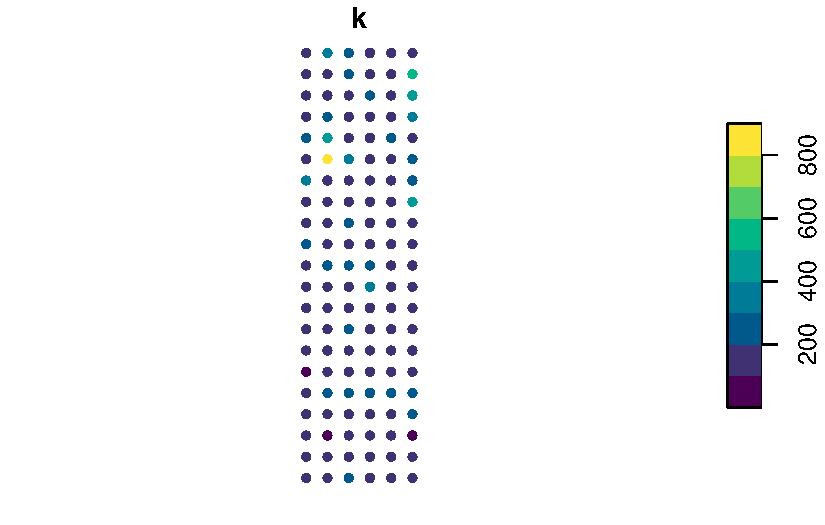
\includegraphics{geo-hw-spdep_files/figure-pdf/unnamed-chunk-2-1.pdf}

}

\end{figure}

\hypertarget{problem-2-using-gstat}{%
\section{\texorpdfstring{Problem 2 (Using
\textbf{gstat})}{Problem 2 (Using gstat)}}\label{problem-2-using-gstat}}

\hypertarget{a}{%
\subsection{(a)}\label{a}}

Create a \texttt{gstat} variogram object. The cutoff distance should be
600. The width of each lag interval should be the cutoff distance
divided by 16. Plot this object. Does the semivariogram seem to have a
well-defined structure? If so, what are the sill, nugget effect, and
range, approximately?

\textbf{Solution}

\begin{Shaded}
\begin{Highlighting}[]
\CommentTok{\# compute empirical semivariogram}
\NormalTok{vhat }\OtherTok{=} \FunctionTok{variogram}\NormalTok{(gsox, }\AttributeTok{cutoff =} \DecValTok{600}\NormalTok{, }\AttributeTok{width =} \DecValTok{600}\SpecialCharTok{/}\DecValTok{16}\NormalTok{)}
\FunctionTok{plot}\NormalTok{(vhat)}
\end{Highlighting}
\end{Shaded}

\begin{figure}[H]

{\centering 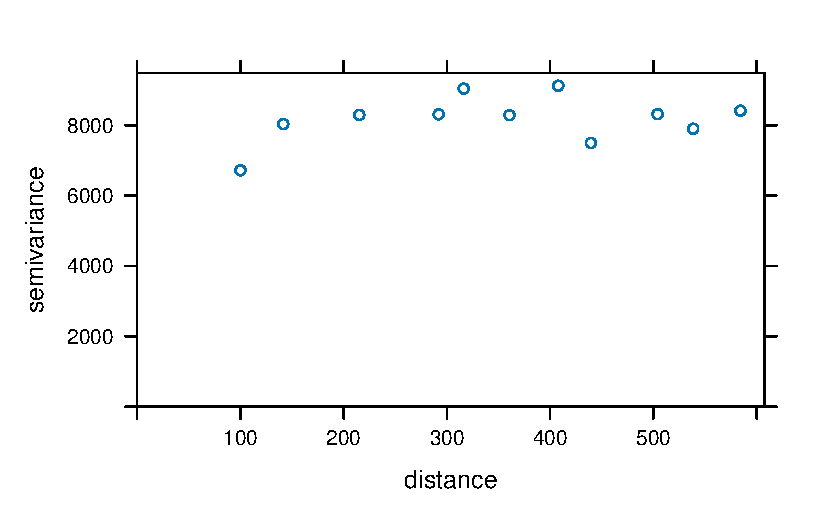
\includegraphics{geo-hw-spdep_files/figure-pdf/unnamed-chunk-3-1.pdf}

}

\end{figure}

\begin{quote}
The semivariogram has some definition and we can identify the nugget
effect as about 6400, the sill appears to be just over 8000, and the
range looks to be about 200.
\end{quote}

\hypertarget{b}{%
\subsection{(b)}\label{b}}

Fit exponential, spherical, and Matern semivariogram models to the
empirical semivariogram in (a) using WRSS. Use
\texttt{fit.kappa\ =\ TRUE} for the Matern model to estimate the
associated smoothness parameter.

Use a table to summarize the estimated partial sill, range parameter,
and nugget for each model. What is the estimated smoothness parameter
for the Matern model?

\textbf{Solution}

\begin{Shaded}
\begin{Highlighting}[]
\CommentTok{\# declaring an empty data frame }
\NormalTok{result }\OtherTok{\textless{}{-}} \FunctionTok{data.frame}\NormalTok{(}\AttributeTok{model =} \FunctionTok{character}\NormalTok{(), }
                 \AttributeTok{psill =} \FunctionTok{double}\NormalTok{(), }
                 \AttributeTok{range =} \FunctionTok{double}\NormalTok{(),}
                 \AttributeTok{wrss =} \FunctionTok{double}\NormalTok{(),}
                 \AttributeTok{stringsAsFactors =} \ConstantTok{FALSE}\NormalTok{) }
  
\CommentTok{\# print the data frame }
\CommentTok{\# str(df)}
\CommentTok{\# result = as.data.frame(colnames(list(\textquotesingle{}model\textquotesingle{},\textquotesingle{}psill\textquotesingle{},\textquotesingle{}range\textquotesingle{},\textquotesingle{}wrss\textquotesingle{})))}
\CommentTok{\# exponential}
\NormalTok{fitexp }\OtherTok{=} \FunctionTok{fit.variogram}\NormalTok{(vhat,}
                       \FunctionTok{vgm}\NormalTok{( }\StringTok{"Exp"}\NormalTok{, }\AttributeTok{range=}\DecValTok{200}\NormalTok{, }\AttributeTok{nugget=}\DecValTok{6400}\NormalTok{),}
                       \AttributeTok{fit.method =} \DecValTok{2}\NormalTok{)}

\FunctionTok{plot}\NormalTok{(vhat, fitexp, }\AttributeTok{main =} \StringTok{"WRSS exponential fit"}\NormalTok{)}
\end{Highlighting}
\end{Shaded}

\begin{figure}[H]

{\centering 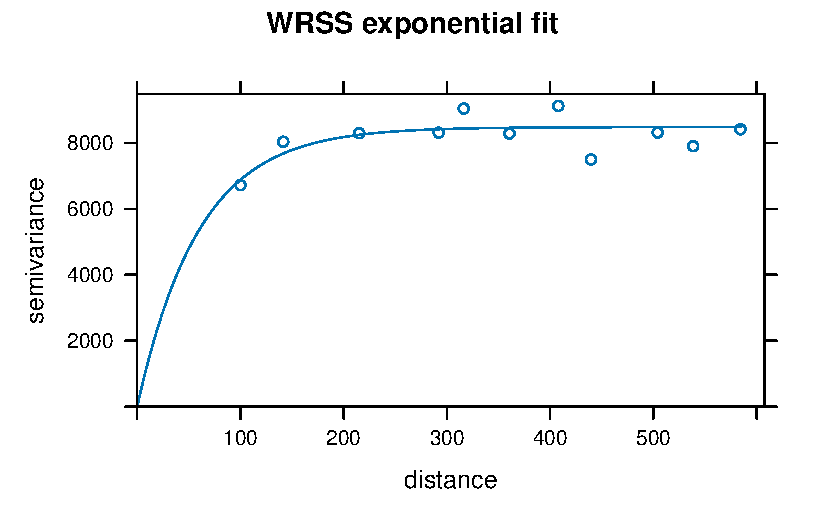
\includegraphics{geo-hw-spdep_files/figure-pdf/unnamed-chunk-4-1.pdf}

}

\end{figure}

\begin{Shaded}
\begin{Highlighting}[]
\NormalTok{rss1 }\OtherTok{=} \FunctionTok{attr}\NormalTok{(fitexp, }\StringTok{"SSErr"}\NormalTok{) }\CommentTok{\# wrss of fit}

\NormalTok{result[}\DecValTok{1}\NormalTok{,}\StringTok{"model"}\NormalTok{] }\OtherTok{=} \StringTok{"Exp"}
\NormalTok{result[}\DecValTok{1}\NormalTok{,}\StringTok{"psill"}\NormalTok{] }\OtherTok{=}\NormalTok{ fitexp[}\DecValTok{2}\NormalTok{,}\StringTok{"psill"}\NormalTok{]}
\NormalTok{result[}\DecValTok{1}\NormalTok{,}\StringTok{"range"}\NormalTok{] }\OtherTok{=}\NormalTok{ fitexp[}\DecValTok{2}\NormalTok{,}\StringTok{"range"}\NormalTok{]}
\NormalTok{result[}\DecValTok{1}\NormalTok{,}\StringTok{"wrss"}\NormalTok{] }\OtherTok{=}\NormalTok{ rss1}
\CommentTok{\# result$wrss[1] = rss1}

\CommentTok{\# spherical}
\NormalTok{fitsphere }\OtherTok{=} \FunctionTok{fit.variogram}\NormalTok{(vhat,}
                       \FunctionTok{vgm}\NormalTok{(}\DecValTok{1600}\NormalTok{, }\StringTok{"Sph"}\NormalTok{, }\DecValTok{200}\NormalTok{, }\DecValTok{6400}\NormalTok{),}
                       \AttributeTok{fit.method =} \DecValTok{2}\NormalTok{)}

\FunctionTok{plot}\NormalTok{(vhat, fitsphere, }\AttributeTok{main =} \StringTok{"Spherical"}\NormalTok{)}
\end{Highlighting}
\end{Shaded}

\begin{figure}[H]

{\centering 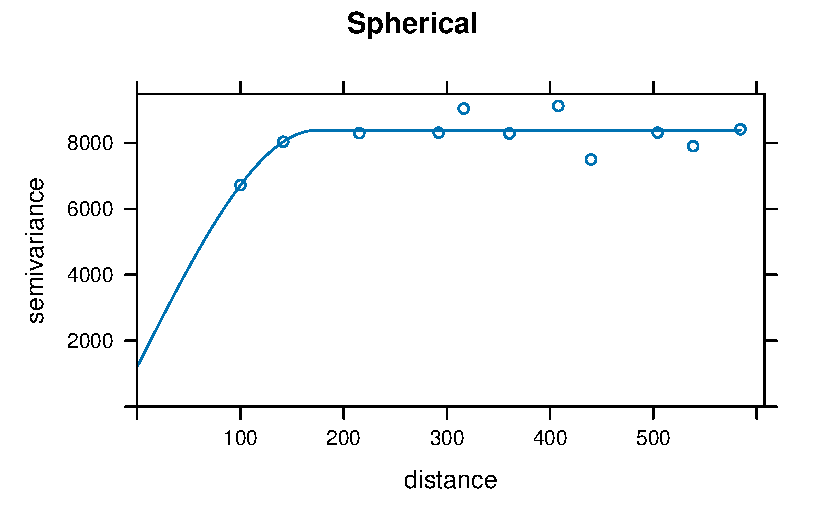
\includegraphics{geo-hw-spdep_files/figure-pdf/unnamed-chunk-4-2.pdf}

}

\end{figure}

\begin{Shaded}
\begin{Highlighting}[]
\NormalTok{rss2 }\OtherTok{=} \FunctionTok{attr}\NormalTok{(fitsphere, }\StringTok{"SSErr"}\NormalTok{) }\CommentTok{\# wrss of fit}

\NormalTok{result[}\DecValTok{2}\NormalTok{,}\StringTok{"model"}\NormalTok{] }\OtherTok{=} \StringTok{"Sph"}
\NormalTok{result[}\DecValTok{2}\NormalTok{,}\StringTok{"psill"}\NormalTok{] }\OtherTok{=}\NormalTok{ fitsphere[}\DecValTok{2}\NormalTok{,}\StringTok{"psill"}\NormalTok{]}
\NormalTok{result[}\DecValTok{2}\NormalTok{,}\StringTok{"range"}\NormalTok{] }\OtherTok{=}\NormalTok{ fitsphere[}\DecValTok{2}\NormalTok{,}\StringTok{"range"}\NormalTok{]}
\NormalTok{result[}\DecValTok{2}\NormalTok{,}\StringTok{"wrss"}\NormalTok{] }\OtherTok{=}\NormalTok{ rss2}
\CommentTok{\# result$wrss[2] = rss2}

\CommentTok{\# matern}
\NormalTok{fitmat }\OtherTok{=} \FunctionTok{fit.variogram}\NormalTok{(vhat,}
                       \FunctionTok{vgm}\NormalTok{(}\DecValTok{1600}\NormalTok{, }\StringTok{"Mat"}\NormalTok{, }\DecValTok{200}\NormalTok{, }\DecValTok{6400}\NormalTok{),}
                       \AttributeTok{fit.method =} \DecValTok{2}\NormalTok{,}\AttributeTok{fit.kappa =} \ConstantTok{TRUE}\NormalTok{)}
\end{Highlighting}
\end{Shaded}

\begin{verbatim}
Warning in fit.variogram(o, m, fit.kappa = FALSE, fit.method = fit.method, :
singular model in variogram fit

Warning in fit.variogram(o, m, fit.kappa = FALSE, fit.method = fit.method, :
singular model in variogram fit

Warning in fit.variogram(o, m, fit.kappa = FALSE, fit.method = fit.method, :
singular model in variogram fit

Warning in fit.variogram(o, m, fit.kappa = FALSE, fit.method = fit.method, :
singular model in variogram fit

Warning in fit.variogram(o, m, fit.kappa = FALSE, fit.method = fit.method, :
singular model in variogram fit

Warning in fit.variogram(o, m, fit.kappa = FALSE, fit.method = fit.method, :
singular model in variogram fit

Warning in fit.variogram(o, m, fit.kappa = FALSE, fit.method = fit.method, :
singular model in variogram fit

Warning in fit.variogram(o, m, fit.kappa = FALSE, fit.method = fit.method, :
singular model in variogram fit

Warning in fit.variogram(o, m, fit.kappa = FALSE, fit.method = fit.method, :
singular model in variogram fit
\end{verbatim}

\begin{verbatim}
Warning in fit.variogram(object, model, fit.sills = fit.sills, fit.ranges =
fit.ranges, : singular model in variogram fit
\end{verbatim}

\begin{verbatim}
Warning in fit.variogram(o, m, fit.kappa = FALSE, fit.method = fit.method, :
singular model in variogram fit
\end{verbatim}

\begin{verbatim}
Warning in fit.variogram(object, model, fit.sills = fit.sills, fit.ranges =
fit.ranges, : singular model in variogram fit
\end{verbatim}

\begin{verbatim}
Warning in fit.variogram(o, m, fit.kappa = FALSE, fit.method = fit.method, :
singular model in variogram fit
\end{verbatim}

\begin{verbatim}
Warning in fit.variogram(object, model, fit.sills = fit.sills, fit.ranges =
fit.ranges, : singular model in variogram fit
\end{verbatim}

\begin{verbatim}
Warning in fit.variogram(o, m, fit.kappa = FALSE, fit.method = fit.method, :
singular model in variogram fit
\end{verbatim}

\begin{verbatim}
Warning in fit.variogram(object, model, fit.sills = fit.sills, fit.ranges =
fit.ranges, : singular model in variogram fit
\end{verbatim}

\begin{verbatim}
Warning in fit.variogram(o, m, fit.kappa = FALSE, fit.method = fit.method, :
singular model in variogram fit
\end{verbatim}

\begin{verbatim}
Warning in fit.variogram(object, model, fit.sills = fit.sills, fit.ranges =
fit.ranges, : singular model in variogram fit
\end{verbatim}

\begin{verbatim}
Warning in fit.variogram(o, m, fit.kappa = FALSE, fit.method = fit.method, :
singular model in variogram fit
\end{verbatim}

\begin{verbatim}
Warning in fit.variogram(object, model, fit.sills = fit.sills, fit.ranges =
fit.ranges, : singular model in variogram fit
\end{verbatim}

\begin{verbatim}
Warning in fit.variogram(o, m, fit.kappa = FALSE, fit.method = fit.method, :
singular model in variogram fit
\end{verbatim}

\begin{verbatim}
Warning in fit.variogram(object, model, fit.sills = fit.sills, fit.ranges =
fit.ranges, : singular model in variogram fit
\end{verbatim}

\begin{verbatim}
Warning in fit.variogram(o, m, fit.kappa = FALSE, fit.method = fit.method, :
singular model in variogram fit
\end{verbatim}

\begin{verbatim}
Warning in fit.variogram(object, model, fit.sills = fit.sills, fit.ranges =
fit.ranges, : singular model in variogram fit
\end{verbatim}

\begin{verbatim}
Warning in fit.variogram(o, m, fit.kappa = FALSE, fit.method = fit.method, :
singular model in variogram fit
\end{verbatim}

\begin{verbatim}
Warning in fit.variogram(object, model, fit.sills = fit.sills, fit.ranges =
fit.ranges, : singular model in variogram fit
\end{verbatim}

\begin{verbatim}
Warning in fit.variogram(o, m, fit.kappa = FALSE, fit.method = fit.method, :
singular model in variogram fit
\end{verbatim}

\begin{verbatim}
Warning in fit.variogram(object, model, fit.sills = fit.sills, fit.ranges =
fit.ranges, : singular model in variogram fit
\end{verbatim}

\begin{verbatim}
Warning in fit.variogram(o, m, fit.kappa = FALSE, fit.method = fit.method, :
singular model in variogram fit

Warning in fit.variogram(o, m, fit.kappa = FALSE, fit.method = fit.method, :
singular model in variogram fit
\end{verbatim}

\begin{verbatim}
Warning in fit.variogram(object, model, fit.sills = fit.sills, fit.ranges =
fit.ranges, : singular model in variogram fit
\end{verbatim}

\begin{verbatim}
Warning in fit.variogram(o, m, fit.kappa = FALSE, fit.method = fit.method, : No
convergence after 200 iterations: try different initial values?
\end{verbatim}

\begin{verbatim}
Warning in fit.variogram(o, m, fit.kappa = FALSE, fit.method = fit.method, :
singular model in variogram fit

Warning in fit.variogram(o, m, fit.kappa = FALSE, fit.method = fit.method, :
singular model in variogram fit

Warning in fit.variogram(o, m, fit.kappa = FALSE, fit.method = fit.method, :
singular model in variogram fit

Warning in fit.variogram(o, m, fit.kappa = FALSE, fit.method = fit.method, :
singular model in variogram fit

Warning in fit.variogram(o, m, fit.kappa = FALSE, fit.method = fit.method, :
singular model in variogram fit

Warning in fit.variogram(o, m, fit.kappa = FALSE, fit.method = fit.method, :
singular model in variogram fit

Warning in fit.variogram(o, m, fit.kappa = FALSE, fit.method = fit.method, :
singular model in variogram fit

Warning in fit.variogram(o, m, fit.kappa = FALSE, fit.method = fit.method, :
singular model in variogram fit
\end{verbatim}

\begin{verbatim}
Warning in fit.variogram(object, model, fit.sills = fit.sills, fit.ranges =
fit.ranges, : singular model in variogram fit
\end{verbatim}

\begin{verbatim}
Warning in fit.variogram(o, m, fit.kappa = FALSE, fit.method = fit.method, :
singular model in variogram fit
\end{verbatim}

\begin{verbatim}
Warning in fit.variogram(object, model, fit.sills = fit.sills, fit.ranges =
fit.ranges, : singular model in variogram fit
\end{verbatim}

\begin{verbatim}
Warning in fit.variogram(o, m, fit.kappa = FALSE, fit.method = fit.method, :
singular model in variogram fit
\end{verbatim}

\begin{verbatim}
Warning in fit.variogram(object, model, fit.sills = fit.sills, fit.ranges =
fit.ranges, : singular model in variogram fit
\end{verbatim}

\begin{verbatim}
Warning in fit.variogram(o, m, fit.kappa = FALSE, fit.method = fit.method, :
singular model in variogram fit
\end{verbatim}

\begin{verbatim}
Warning in fit.variogram(object, model, fit.sills = fit.sills, fit.ranges =
fit.ranges, : singular model in variogram fit
\end{verbatim}

\begin{verbatim}
Warning in fit.variogram(o, m, fit.kappa = FALSE, fit.method = fit.method, :
singular model in variogram fit
\end{verbatim}

\begin{verbatim}
Warning in fit.variogram(object, model, fit.sills = fit.sills, fit.ranges =
fit.ranges, : singular model in variogram fit
\end{verbatim}

\begin{verbatim}
Warning in fit.variogram(o, m, fit.kappa = FALSE, fit.method = fit.method, :
singular model in variogram fit
\end{verbatim}

\begin{verbatim}
Warning in fit.variogram(object, model, fit.sills = fit.sills, fit.ranges =
fit.ranges, : singular model in variogram fit
\end{verbatim}

\begin{verbatim}
Warning in fit.variogram(o, m, fit.kappa = FALSE, fit.method = fit.method, :
singular model in variogram fit
\end{verbatim}

\begin{verbatim}
Warning in fit.variogram(object, model, fit.sills = fit.sills, fit.ranges =
fit.ranges, : singular model in variogram fit
\end{verbatim}

\begin{verbatim}
Warning in fit.variogram(o, m, fit.kappa = FALSE, fit.method = fit.method, :
singular model in variogram fit
\end{verbatim}

\begin{verbatim}
Warning in fit.variogram(object, model, fit.sills = fit.sills, fit.ranges =
fit.ranges, : singular model in variogram fit
\end{verbatim}

\begin{verbatim}
Warning in fit.variogram(o, m, fit.kappa = FALSE, fit.method = fit.method, :
singular model in variogram fit
\end{verbatim}

\begin{verbatim}
Warning in fit.variogram(object, model, fit.sills = fit.sills, fit.ranges =
fit.ranges, : singular model in variogram fit
\end{verbatim}

\begin{verbatim}
Warning in fit.variogram(o, m, fit.kappa = FALSE, fit.method = fit.method, :
singular model in variogram fit
\end{verbatim}

\begin{verbatim}
Warning in fit.variogram(object, model, fit.sills = fit.sills, fit.ranges =
fit.ranges, : singular model in variogram fit
\end{verbatim}

\begin{verbatim}
Warning in fit.variogram(o, m, fit.kappa = FALSE, fit.method = fit.method, : No
convergence after 200 iterations: try different initial values?
\end{verbatim}

\begin{verbatim}
Warning in fit.variogram(object, model, fit.sills = fit.sills, fit.ranges =
fit.ranges, : singular model in variogram fit
\end{verbatim}

\begin{verbatim}
Warning in fit.variogram(o, m, fit.kappa = FALSE, fit.method = fit.method, :
singular model in variogram fit

Warning in fit.variogram(o, m, fit.kappa = FALSE, fit.method = fit.method, :
singular model in variogram fit

Warning in fit.variogram(o, m, fit.kappa = FALSE, fit.method = fit.method, :
singular model in variogram fit

Warning in fit.variogram(o, m, fit.kappa = FALSE, fit.method = fit.method, :
singular model in variogram fit

Warning in fit.variogram(o, m, fit.kappa = FALSE, fit.method = fit.method, :
singular model in variogram fit

Warning in fit.variogram(o, m, fit.kappa = FALSE, fit.method = fit.method, :
singular model in variogram fit
\end{verbatim}

\begin{verbatim}
Warning in fit.variogram(object, model, fit.sills = fit.sills, fit.ranges =
fit.ranges, : singular model in variogram fit
\end{verbatim}

\begin{verbatim}
Warning in fit.variogram(o, m, fit.kappa = FALSE, fit.method = fit.method, :
singular model in variogram fit
\end{verbatim}

\begin{verbatim}
Warning in fit.variogram(object, model, fit.sills = fit.sills, fit.ranges =
fit.ranges, : singular model in variogram fit
\end{verbatim}

\begin{Shaded}
\begin{Highlighting}[]
\FunctionTok{plot}\NormalTok{(vhat, fitmat, }\AttributeTok{main =} \StringTok{"Matern"}\NormalTok{)}
\end{Highlighting}
\end{Shaded}

\begin{figure}[H]

{\centering 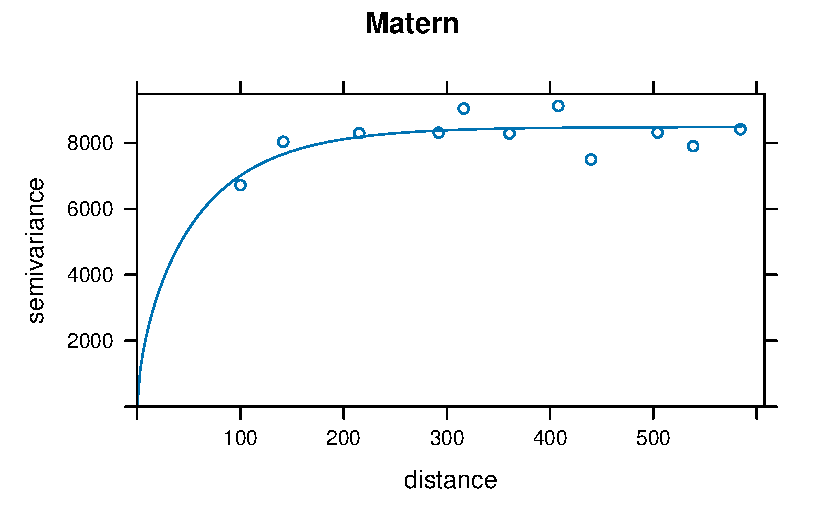
\includegraphics{geo-hw-spdep_files/figure-pdf/unnamed-chunk-4-3.pdf}

}

\end{figure}

\begin{Shaded}
\begin{Highlighting}[]
\NormalTok{rss3 }\OtherTok{=} \FunctionTok{attr}\NormalTok{(fitmat, }\StringTok{"SSErr"}\NormalTok{) }\CommentTok{\# wrss of fit}

\NormalTok{result[}\DecValTok{3}\NormalTok{,}\StringTok{"model"}\NormalTok{] }\OtherTok{=} \StringTok{"Mat"}
\NormalTok{result[}\DecValTok{3}\NormalTok{,}\StringTok{"psill"}\NormalTok{] }\OtherTok{=}\NormalTok{ fitmat[}\DecValTok{2}\NormalTok{,}\StringTok{"psill"}\NormalTok{]}
\NormalTok{result[}\DecValTok{3}\NormalTok{,}\StringTok{"range"}\NormalTok{] }\OtherTok{=}\NormalTok{ fitmat[}\DecValTok{2}\NormalTok{,}\StringTok{"range"}\NormalTok{]}
\NormalTok{result[}\DecValTok{3}\NormalTok{,}\StringTok{"wrss"}\NormalTok{] }\OtherTok{=}\NormalTok{ rss3}
\CommentTok{\# result$wrss[3] = rss3}

\NormalTok{result}
\end{Highlighting}
\end{Shaded}

\begin{verbatim}
  model    psill     range       wrss
1   Exp 8479.252  59.96227  0.3181106
2   Sph 7174.180 173.76091 10.1002295
3   Mat 8480.321  78.77511  0.1070215
\end{verbatim}

\begin{quote}
the estimated smoothness for the Matern model is 0.107
\end{quote}

\hypertarget{c}{%
\subsection{(c)}\label{c}}

In one plot, overlay each fitted variogram model from (c) to the
empirical semivariogram found in (b). Note: You will need to extract the
relevant information from your gstat variogram object. Also, you will
probably want to use the \texttt{variogramLine} function to obtain
values for the theoretical models of each fitted model. Use this
information to construct a single plot with the empirical semivariogram
and the fitted models, making sure to label each model properly.

\textbf{Solution}

\begin{Shaded}
\begin{Highlighting}[]
\FunctionTok{library}\NormalTok{(ggplot2)}

\NormalTok{vhat }\OtherTok{=} \FunctionTok{variogram}\NormalTok{(gsox, }\AttributeTok{cutoff =} \DecValTok{600}\NormalTok{, }\AttributeTok{width =} \DecValTok{600}\SpecialCharTok{/}\DecValTok{16}\NormalTok{)}
\NormalTok{exp\_line }\OtherTok{=} \FunctionTok{variogramLine}\NormalTok{(fitexp,}\AttributeTok{maxdist =} \FunctionTok{max}\NormalTok{(vhat}\SpecialCharTok{$}\NormalTok{dist))}
\NormalTok{sph\_line }\OtherTok{=} \FunctionTok{variogramLine}\NormalTok{(fitsphere,}\AttributeTok{maxdist =} \FunctionTok{max}\NormalTok{(vhat}\SpecialCharTok{$}\NormalTok{dist))}
\NormalTok{mat\_line }\OtherTok{=} \FunctionTok{variogramLine}\NormalTok{(fitmat,}\AttributeTok{maxdist =} \FunctionTok{max}\NormalTok{(vhat}\SpecialCharTok{$}\NormalTok{dist))}


\FunctionTok{ggplot}\NormalTok{()}\SpecialCharTok{+}
  \FunctionTok{geom\_point}\NormalTok{(vhat, }\AttributeTok{mapping=}\FunctionTok{aes}\NormalTok{(}\AttributeTok{x=}\NormalTok{dist,}\AttributeTok{y=}\NormalTok{gamma,}\AttributeTok{color=}\StringTok{\textquotesingle{}red\textquotesingle{}}\NormalTok{))}\SpecialCharTok{+}
  \FunctionTok{geom\_line}\NormalTok{(exp\_line,}\AttributeTok{mapping=}\FunctionTok{aes}\NormalTok{(}\AttributeTok{x=}\NormalTok{dist,}\AttributeTok{y=}\NormalTok{gamma,}\AttributeTok{color=}\StringTok{\textquotesingle{}darkgreen\textquotesingle{}}\NormalTok{))}\SpecialCharTok{+}
  \FunctionTok{geom\_line}\NormalTok{(sph\_line,}\AttributeTok{mapping=}\FunctionTok{aes}\NormalTok{(}\AttributeTok{x=}\NormalTok{dist,}\AttributeTok{y=}\NormalTok{gamma,}\AttributeTok{color=}\StringTok{\textquotesingle{}orange\textquotesingle{}}\NormalTok{))}\SpecialCharTok{+}
  \FunctionTok{geom\_line}\NormalTok{(mat\_line,}\AttributeTok{mapping=}\FunctionTok{aes}\NormalTok{(}\AttributeTok{x=}\NormalTok{dist,}\AttributeTok{y=}\NormalTok{gamma,}\AttributeTok{color=}\StringTok{\textquotesingle{}darkblue\textquotesingle{}}\NormalTok{))}\SpecialCharTok{+}
  \FunctionTok{scale\_colour\_manual}\NormalTok{(}\AttributeTok{name =} \StringTok{\textquotesingle{}Variogram Model\textquotesingle{}}\NormalTok{,}\AttributeTok{aesthetics =} \StringTok{"color"}\NormalTok{,}
                      \AttributeTok{values=}\FunctionTok{c}\NormalTok{(}\StringTok{\textquotesingle{}red\textquotesingle{}}\OtherTok{=}\StringTok{\textquotesingle{}red\textquotesingle{}}\NormalTok{,}
                               \StringTok{\textquotesingle{}darkgreen\textquotesingle{}}\OtherTok{=}\StringTok{\textquotesingle{}darkgreen\textquotesingle{}}\NormalTok{,}
                               \StringTok{\textquotesingle{}orange\textquotesingle{}}\OtherTok{=}\StringTok{\textquotesingle{}orange\textquotesingle{}}\NormalTok{,}
                               \StringTok{\textquotesingle{}darkblue\textquotesingle{}}\OtherTok{=}\StringTok{\textquotesingle{}darkblue\textquotesingle{}}\NormalTok{),}
                      \AttributeTok{labels =} \FunctionTok{c}\NormalTok{(}\StringTok{\textquotesingle{}Mat\textquotesingle{}}\NormalTok{,}\StringTok{\textquotesingle{}Exp\textquotesingle{}}\NormalTok{,}\StringTok{\textquotesingle{}Sph\textquotesingle{}}\NormalTok{,}\StringTok{\textquotesingle{}vhat\textquotesingle{}}\NormalTok{))}
\end{Highlighting}
\end{Shaded}

\begin{figure}[H]

{\centering 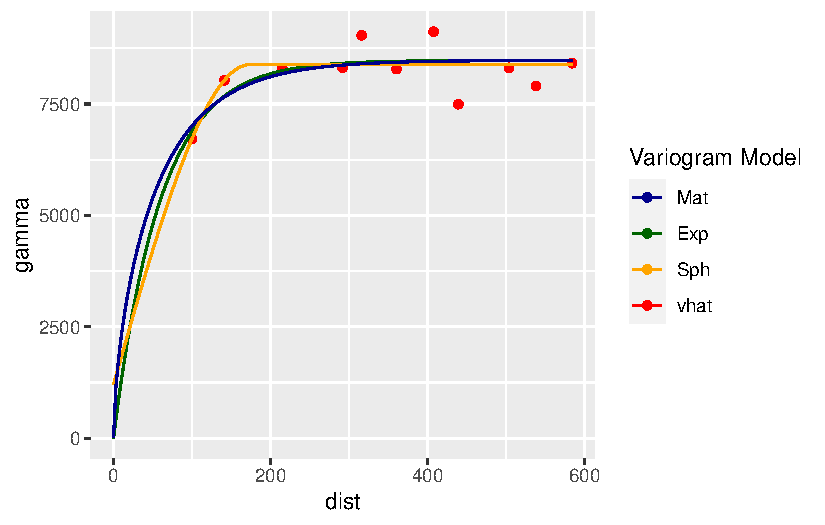
\includegraphics{geo-hw-spdep_files/figure-pdf/unnamed-chunk-5-1.pdf}

}

\end{figure}

\hypertarget{problem-3-using-geor}{%
\section{\texorpdfstring{Problem 3 (Using
\textbf{geoR})}{Problem 3 (Using geoR)}}\label{problem-3-using-geor}}

\hypertarget{a-1}{%
\subsection{(a)}\label{a-1}}

Use the geoR \texttt{variog} function to create an empirical
semivariogram. The \texttt{max.dist} value should be the same as the
cutoff from Problem 2. Use 20 lag intervals. Plot this object.

\textbf{Solution}

\begin{Shaded}
\begin{Highlighting}[]
\FunctionTok{library}\NormalTok{(geoR)}

\CommentTok{\# load smoky dataframe}
\FunctionTok{load}\NormalTok{(}\StringTok{"ox.rda"}\NormalTok{)}

\CommentTok{\# create geodata object for geoR}
\NormalTok{geox }\OtherTok{=} \FunctionTok{as.geodata}\NormalTok{(}\FunctionTok{cbind}\NormalTok{(ox}\SpecialCharTok{$}\NormalTok{x, ox}\SpecialCharTok{$}\NormalTok{y, ox}\SpecialCharTok{$}\NormalTok{k))}

\CommentTok{\# estimated semivariogram}
\NormalTok{vhat2 }\OtherTok{=} \FunctionTok{variog}\NormalTok{(geox, }\AttributeTok{max.dist =} \DecValTok{600}\NormalTok{, }\AttributeTok{uvec =} \DecValTok{20}\NormalTok{)}
\end{Highlighting}
\end{Shaded}

\begin{verbatim}
variog: computing omnidirectional variogram
\end{verbatim}

\begin{Shaded}
\begin{Highlighting}[]
\FunctionTok{plot}\NormalTok{(vhat2)}
\end{Highlighting}
\end{Shaded}

\begin{figure}[H]

{\centering 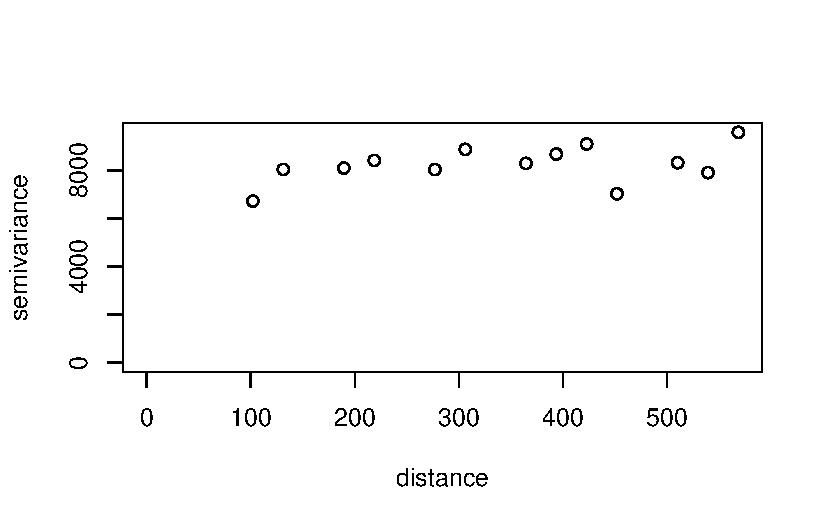
\includegraphics{geo-hw-spdep_files/figure-pdf/unnamed-chunk-6-1.pdf}

}

\end{figure}

\hypertarget{b-1}{%
\subsection{(b)}\label{b-1}}

(Fit exponential, spherical, and Matern variogram models to empirical
semivariogram in (a) using WRSS. Use \texttt{fix.kappa\ =\ FALSE} for
the Matern model to estimate the associated smoothness parameter. Use a
table to summarize the estimated partial sill, range parameter, and
nugget for each model. Provide plots of each fitted variogram model to
the empirical variogram. What is the estimated smoothness parameter for
the Matern model?

\begin{Shaded}
\begin{Highlighting}[]
\NormalTok{result2 }\OtherTok{\textless{}{-}} \FunctionTok{data.frame}\NormalTok{(}\AttributeTok{model =} \FunctionTok{character}\NormalTok{(), }
                 \AttributeTok{psill =} \FunctionTok{double}\NormalTok{(), }
                 \AttributeTok{range\_param =} \FunctionTok{double}\NormalTok{(),}
                 \AttributeTok{wrss =} \FunctionTok{double}\NormalTok{(),}
                 \AttributeTok{stringsAsFactors =} \ConstantTok{FALSE}\NormalTok{)}

\CommentTok{\# fit exponential model using geoR package}
\NormalTok{fitexp }\OtherTok{=} \FunctionTok{variofit}\NormalTok{(vhat2, }\AttributeTok{ini.cov.pars =} \FunctionTok{c}\NormalTok{(}\DecValTok{1600}\NormalTok{, }\DecValTok{200}\NormalTok{),}
                  \AttributeTok{nugget =} \DecValTok{6400}\NormalTok{,}
                  \AttributeTok{cov.model =} \StringTok{"exponential"}\NormalTok{,}
\NormalTok{                  )}
\end{Highlighting}
\end{Shaded}

\begin{verbatim}
variofit: covariance model used is exponential 
variofit: weights used: npairs 
variofit: minimisation function used: optim 
\end{verbatim}

\begin{Shaded}
\begin{Highlighting}[]
\NormalTok{exp\_params1 }\OtherTok{\textless{}{-}}\NormalTok{ fitexp}\SpecialCharTok{$}\NormalTok{cov.pars }
\NormalTok{exp\_c0 }\OtherTok{\textless{}{-}}\NormalTok{ fitexp}\SpecialCharTok{$}\NormalTok{nugget }
\NormalTok{exp\_wrss }\OtherTok{\textless{}{-}}\NormalTok{ fitexp}\SpecialCharTok{$}\NormalTok{value}\SpecialCharTok{/}\DecValTok{2} 

\NormalTok{result2[}\DecValTok{1}\NormalTok{,}\StringTok{"model"}\NormalTok{] }\OtherTok{=} \StringTok{"Exp"}
\NormalTok{result2[}\DecValTok{1}\NormalTok{,}\StringTok{"psill"}\NormalTok{] }\OtherTok{=}\NormalTok{ exp\_params1[[}\DecValTok{1}\NormalTok{]]}
\NormalTok{result2[}\DecValTok{1}\NormalTok{,}\StringTok{"range\_param"}\NormalTok{] }\OtherTok{=}\NormalTok{ exp\_params1[[}\DecValTok{2}\NormalTok{]]}
\NormalTok{result2[}\DecValTok{1}\NormalTok{,}\StringTok{"wrss"}\NormalTok{] }\OtherTok{=}\NormalTok{ exp\_wrss}

\CommentTok{\# fit spherical model using geoR package}
\NormalTok{fit\_sph }\OtherTok{=} \FunctionTok{variofit}\NormalTok{(vhat2, }\AttributeTok{ini.cov.pars =} \FunctionTok{c}\NormalTok{(}\DecValTok{1600}\NormalTok{, }\DecValTok{200}\NormalTok{),}
                  \AttributeTok{nugget =} \DecValTok{6400}\NormalTok{,}
                  \AttributeTok{cov.model =} \StringTok{"spherical"}\NormalTok{,}
\NormalTok{                  )}
\end{Highlighting}
\end{Shaded}

\begin{verbatim}
variofit: covariance model used is spherical 
variofit: weights used: npairs 
variofit: minimisation function used: optim 
\end{verbatim}

\begin{Shaded}
\begin{Highlighting}[]
\NormalTok{sph\_params1 }\OtherTok{\textless{}{-}}\NormalTok{ fit\_sph}\SpecialCharTok{$}\NormalTok{cov.pars }
\NormalTok{sph\_c0 }\OtherTok{\textless{}{-}}\NormalTok{ fit\_sph}\SpecialCharTok{$}\NormalTok{nugget }
\NormalTok{sph\_wrss }\OtherTok{\textless{}{-}}\NormalTok{ fit\_sph}\SpecialCharTok{$}\NormalTok{value}\SpecialCharTok{/}\DecValTok{2} 

\NormalTok{result2[}\DecValTok{2}\NormalTok{,}\StringTok{"model"}\NormalTok{] }\OtherTok{=} \StringTok{"Sph"}
\NormalTok{result2[}\DecValTok{2}\NormalTok{,}\StringTok{"psill"}\NormalTok{] }\OtherTok{=}\NormalTok{ sph\_params1[[}\DecValTok{1}\NormalTok{]]}
\NormalTok{result2[}\DecValTok{2}\NormalTok{,}\StringTok{"range\_param"}\NormalTok{] }\OtherTok{=}\NormalTok{ sph\_params1[[}\DecValTok{2}\NormalTok{]]}
\NormalTok{result2[}\DecValTok{2}\NormalTok{,}\StringTok{"wrss"}\NormalTok{] }\OtherTok{=}\NormalTok{ sph\_wrss}

\CommentTok{\# fit matern model}
\NormalTok{fit\_mat }\OtherTok{=} \FunctionTok{variofit}\NormalTok{(vhat2, }\AttributeTok{ini.cov.pars =} \FunctionTok{c}\NormalTok{(}\DecValTok{1600}\NormalTok{, }\DecValTok{200}\NormalTok{),}
                  \AttributeTok{nugget =} \DecValTok{6400}\NormalTok{,}
                  \AttributeTok{cov.model =} \StringTok{"matern"}\NormalTok{,}
                  \AttributeTok{fix.kappa =} \ConstantTok{FALSE}
\NormalTok{                  )}
\end{Highlighting}
\end{Shaded}

\begin{verbatim}
variofit: covariance model used is matern 
variofit: weights used: npairs 
variofit: minimisation function used: optim 
\end{verbatim}

\begin{verbatim}
Warning in cov.spatial(g.l$u, cov.model = g.l$cov.model, kappa = kappa, :
Infinity value in cov.spatial

Warning in cov.spatial(g.l$u, cov.model = g.l$cov.model, kappa = kappa, :
Infinity value in cov.spatial

Warning in cov.spatial(g.l$u, cov.model = g.l$cov.model, kappa = kappa, :
Infinity value in cov.spatial

Warning in cov.spatial(g.l$u, cov.model = g.l$cov.model, kappa = kappa, :
Infinity value in cov.spatial

Warning in cov.spatial(g.l$u, cov.model = g.l$cov.model, kappa = kappa, :
Infinity value in cov.spatial

Warning in cov.spatial(g.l$u, cov.model = g.l$cov.model, kappa = kappa, :
Infinity value in cov.spatial

Warning in cov.spatial(g.l$u, cov.model = g.l$cov.model, kappa = kappa, :
Infinity value in cov.spatial

Warning in cov.spatial(g.l$u, cov.model = g.l$cov.model, kappa = kappa, :
Infinity value in cov.spatial

Warning in cov.spatial(g.l$u, cov.model = g.l$cov.model, kappa = kappa, :
Infinity value in cov.spatial
\end{verbatim}

\begin{Shaded}
\begin{Highlighting}[]
\NormalTok{mat\_params1 }\OtherTok{\textless{}{-}}\NormalTok{ fit\_mat}\SpecialCharTok{$}\NormalTok{cov.pars }
\NormalTok{mat\_c0 }\OtherTok{\textless{}{-}}\NormalTok{ fit\_mat}\SpecialCharTok{$}\NormalTok{nugget }
\NormalTok{mat\_wrss }\OtherTok{\textless{}{-}}\NormalTok{ fit\_mat}\SpecialCharTok{$}\NormalTok{value}\SpecialCharTok{/}\DecValTok{2} 

\NormalTok{result2[}\DecValTok{3}\NormalTok{,}\StringTok{"model"}\NormalTok{] }\OtherTok{=} \StringTok{"Exp"}
\NormalTok{result2[}\DecValTok{3}\NormalTok{,}\StringTok{"psill"}\NormalTok{] }\OtherTok{=}\NormalTok{ mat\_params1[[}\DecValTok{1}\NormalTok{]]}
\NormalTok{result2[}\DecValTok{3}\NormalTok{,}\StringTok{"range\_param"}\NormalTok{] }\OtherTok{=}\NormalTok{ mat\_params1[[}\DecValTok{2}\NormalTok{]]}
\NormalTok{result2[}\DecValTok{3}\NormalTok{,}\StringTok{"wrss"}\NormalTok{] }\OtherTok{=}\NormalTok{ mat\_wrss}
\end{Highlighting}
\end{Shaded}

\hypertarget{c-1}{%
\subsection{(c)}\label{c-1}}

In one plot, overlay each fitted variogram model from (b) to the
empirical semivariogram found in (a). Making sure to label each model
properly.

\textbf{Solution}

\begin{Shaded}
\begin{Highlighting}[]
\FunctionTok{plot}\NormalTok{(vhat2}\SpecialCharTok{$}\NormalTok{u,vhat2}\SpecialCharTok{$}\NormalTok{v,}\AttributeTok{col=}\StringTok{\textquotesingle{}red\textquotesingle{}}\NormalTok{)}
\NormalTok{geoR}\SpecialCharTok{:::}\FunctionTok{lines.variomodel.variofit}\NormalTok{(fitexp,}\AttributeTok{col=}\StringTok{\textquotesingle{}green\textquotesingle{}}\NormalTok{)}
\NormalTok{geoR}\SpecialCharTok{:::}\FunctionTok{lines.variomodel.variofit}\NormalTok{(fit\_sph,}\AttributeTok{col=}\StringTok{\textquotesingle{}blue\textquotesingle{}}\NormalTok{)}
\NormalTok{geoR}\SpecialCharTok{:::}\FunctionTok{lines.variomodel.variofit}\NormalTok{(fit\_mat,}\AttributeTok{col=}\StringTok{\textquotesingle{}orange\textquotesingle{}}\NormalTok{)}
\end{Highlighting}
\end{Shaded}

\begin{figure}[H]

{\centering 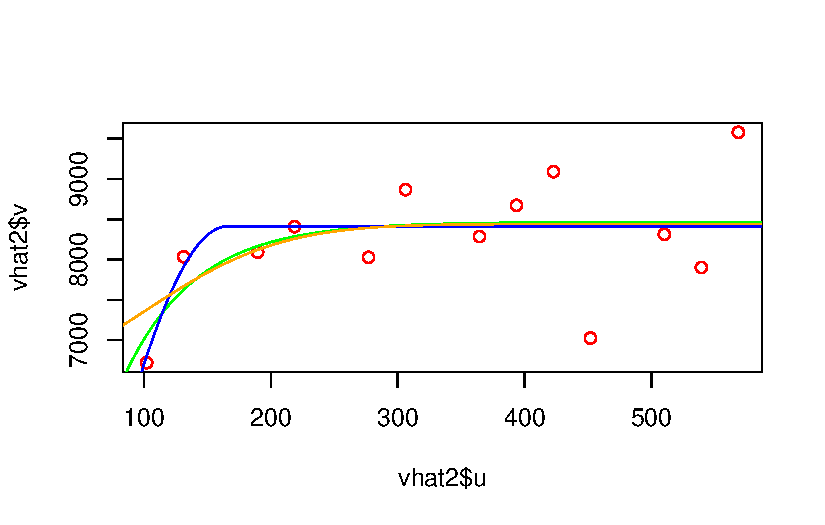
\includegraphics{geo-hw-spdep_files/figure-pdf/unnamed-chunk-8-1.pdf}

}

\end{figure}

\hypertarget{d}{%
\subsection{(d)}\label{d}}

Use the \texttt{variog4} function to create a directional semivariogram
(using the default direction). Set \texttt{maxdist} to be 600. Use 10
bins. Plot this object. What kind of anisotropy does this appear to be?
Why? (Note that there are few observations in certain bins, so there may
be some ``missing'' data).

\textbf{Solution}

\begin{Shaded}
\begin{Highlighting}[]
\NormalTok{dv }\OtherTok{\textless{}{-}} \FunctionTok{variog4}\NormalTok{(geox,}\AttributeTok{uvec=}\DecValTok{10}\NormalTok{,}\AttributeTok{max.dist =} \DecValTok{600}\NormalTok{)}
\end{Highlighting}
\end{Shaded}

\begin{verbatim}
variog: computing variogram for direction = 0 degrees (0 radians)
        tolerance angle = 22.5 degrees (0.393 radians)
variog: computing variogram for direction = 45 degrees (0.785 radians)
        tolerance angle = 22.5 degrees (0.393 radians)
variog: computing variogram for direction = 90 degrees (1.571 radians)
        tolerance angle = 22.5 degrees (0.393 radians)
variog: computing variogram for direction = 135 degrees (2.356 radians)
        tolerance angle = 22.5 degrees (0.393 radians)
variog: computing omnidirectional variogram
\end{verbatim}

\begin{Shaded}
\begin{Highlighting}[]
\FunctionTok{plot}\NormalTok{(dv)}
\end{Highlighting}
\end{Shaded}

\begin{figure}[H]

{\centering 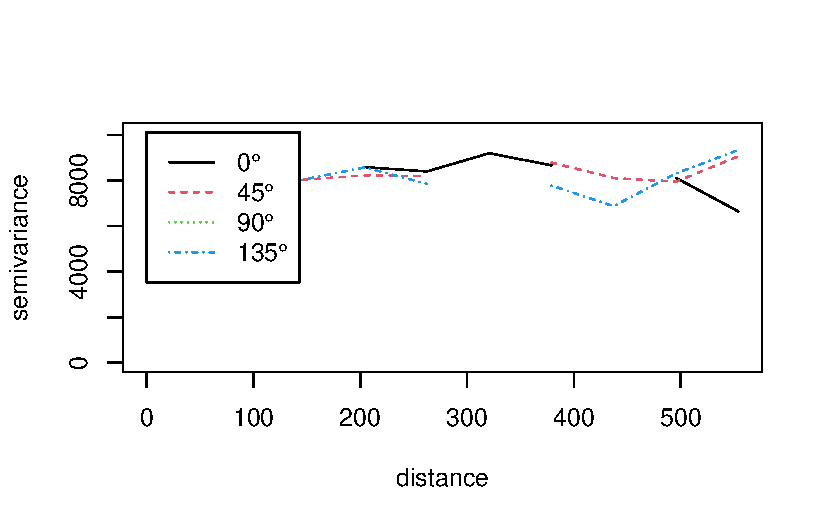
\includegraphics{geo-hw-spdep_files/figure-pdf/unnamed-chunk-9-1.pdf}

}

\end{figure}

\begin{quote}
from the plot, it appears to be geometric anisotropy because the
directional semivariograms have approximately the same shape and sill
but it is hard to compare the range between orthogonal directions, which
would help with the second condition for geometric anisotropy - that the
range in one direction has the max range and the range of the
perpendicular direction would be the min range.
\end{quote}

\hypertarget{e}{%
\subsection{(e)}\label{e}}

Use REML to fit an omnidirectional spherical semivariogram model to the
observed data. Then fit a directional semivariogram model with
\texttt{psiA\ =\ pi/2} and \texttt{psiR\ =\ 1}. Make sure that the
\texttt{psiA} and \texttt{psiR} parameters are not fixed during
estimation for the second parameter. For both models use initial values
of 6000 for the partial sill, 50 for the range parameter, and 1000 for
the nugget. Note: this will take a fair bit of time. Which model should
be preferred, in terms of AIC?

\textbf{Solution}

\hypertarget{problem-3}{%
\section{Problem 3}\label{problem-3}}

Write code to manually construct and plot an omnidirectional
semivariogram for the oxford data. Use 16 lag intervals and a distance
upper bound of 600. Some steps to do this:

\hypertarget{a-2}{%
\subsection{(a)}\label{a-2}}

Create a matrix that describes the indices of all unique pairs of points
\((1, 2), (1, 3), (1, N), (2, 3), .., (2, N), \ldots, (N-1, N)\). Each
row should be a different pair.

\begin{Shaded}
\begin{Highlighting}[]
\CommentTok{\# get x and y vectors, combine into 2d Array}
\NormalTok{vx }\OtherTok{\textless{}{-}}\NormalTok{ ox}\SpecialCharTok{$}\NormalTok{x}
\NormalTok{vy }\OtherTok{\textless{}{-}}\NormalTok{ ox}\SpecialCharTok{$}\NormalTok{y}
\NormalTok{v }\OtherTok{\textless{}{-}} \FunctionTok{cbind}\NormalTok{(vx,vy)}

\CommentTok{\# look at uniqe values for x and y}
\NormalTok{N}\OtherTok{=}\FunctionTok{length}\NormalTok{(}\FunctionTok{unique}\NormalTok{(vx))}
\NormalTok{Z }\OtherTok{=} \FunctionTok{length}\NormalTok{(}\FunctionTok{unique}\NormalTok{(vy))}
\CommentTok{\# N =10}

\CommentTok{\# empty data.frame to store results}
\NormalTok{v\_list }\OtherTok{=} \FunctionTok{data.frame}\NormalTok{()}

\CommentTok{\# instantiate index parameter}
\NormalTok{index }\OtherTok{=} \DecValTok{1}

\CommentTok{\# loop through N{-}1 and generate index points for each unique (x,y) combination}
\ControlFlowTok{for}\NormalTok{ (i }\ControlFlowTok{in} \DecValTok{1}\SpecialCharTok{:}\NormalTok{(N}\DecValTok{{-}1}\NormalTok{))\{}
\NormalTok{  u }\OtherTok{=} \DecValTok{1}
  \ControlFlowTok{while}\NormalTok{ (i}\SpecialCharTok{+}\NormalTok{u}\SpecialCharTok{\textless{}=}\NormalTok{Z)\{}
\NormalTok{    v\_list[index,}\DecValTok{1}\NormalTok{] }\OtherTok{=}\NormalTok{ i}
\NormalTok{    v\_list[index,}\DecValTok{2}\NormalTok{] }\OtherTok{=}\NormalTok{ i}\SpecialCharTok{+}\NormalTok{u}
\NormalTok{    u }\OtherTok{=}\NormalTok{ u}\SpecialCharTok{+}\DecValTok{1}
\NormalTok{    index}\OtherTok{=}\NormalTok{index}\SpecialCharTok{+}\DecValTok{1}
\NormalTok{  \}}
\NormalTok{\}}

\CommentTok{\# convert to matrix and view}
\NormalTok{v\_mat }\OtherTok{=} \FunctionTok{as.matrix}\NormalTok{(}\AttributeTok{x=}\NormalTok{v\_list,}\AttributeTok{nrow=}\NormalTok{index}\DecValTok{{-}1}\NormalTok{,}\AttributeTok{ncol=}\DecValTok{2}\NormalTok{)}
\NormalTok{v\_mat}
\end{Highlighting}
\end{Shaded}

\begin{verbatim}
   V1 V2
1   1  2
2   1  3
3   1  4
4   1  5
5   1  6
6   1  7
7   1  8
8   1  9
9   1 10
10  1 11
11  1 12
12  1 13
13  1 14
14  1 15
15  1 16
16  1 17
17  1 18
18  1 19
19  1 20
20  1 21
21  2  3
22  2  4
23  2  5
24  2  6
25  2  7
26  2  8
27  2  9
28  2 10
29  2 11
30  2 12
31  2 13
32  2 14
33  2 15
34  2 16
35  2 17
36  2 18
37  2 19
38  2 20
39  2 21
40  3  4
41  3  5
42  3  6
43  3  7
44  3  8
45  3  9
46  3 10
47  3 11
48  3 12
49  3 13
50  3 14
51  3 15
52  3 16
53  3 17
54  3 18
55  3 19
56  3 20
57  3 21
58  4  5
59  4  6
60  4  7
61  4  8
62  4  9
63  4 10
64  4 11
65  4 12
66  4 13
67  4 14
68  4 15
69  4 16
70  4 17
71  4 18
72  4 19
73  4 20
74  4 21
75  5  6
76  5  7
77  5  8
78  5  9
79  5 10
80  5 11
81  5 12
82  5 13
83  5 14
84  5 15
85  5 16
86  5 17
87  5 18
88  5 19
89  5 20
90  5 21
\end{verbatim}

\hypertarget{b-2}{%
\subsection{(b)}\label{b-2}}

Compute the distances between all unique pairs of observed points. The
distances for the unique pairs should be stored in a vector (in the same
order as 1). \textbf{Print the range of these distances.}

\begin{Shaded}
\begin{Highlighting}[]
\NormalTok{dv }\OtherTok{\textless{}{-}} \FunctionTok{as.matrix}\NormalTok{(}\FunctionTok{apply}\NormalTok{(v,}\AttributeTok{FUN=}\NormalTok{dist,}\AttributeTok{MARGIN=}\DecValTok{1}\NormalTok{))}
\FunctionTok{range}\NormalTok{(dv)}
\end{Highlighting}
\end{Shaded}

\begin{verbatim}
[1]    0 2000
\end{verbatim}

\hypertarget{c-2}{%
\subsection{(c)}\label{c-2}}

Compute the squared difference between the responses for all unique
pairs of points (in the same order as 1). \textbf{Print the range of the
square response differences}.

\begin{Shaded}
\begin{Highlighting}[]
\CommentTok{\# the following assumes we are referring to the y value as our "response"}

\CommentTok{\# u\_vy \textless{}{-} as.matrix(unique(vy))}
\NormalTok{uv }\OtherTok{\textless{}{-}} \FunctionTok{as.matrix}\NormalTok{(}\FunctionTok{unique}\NormalTok{(v))}
\NormalTok{responses }\OtherTok{=} \FunctionTok{as.matrix}\NormalTok{(uv[,}\DecValTok{2}\NormalTok{])}

\CommentTok{\#result df}
\NormalTok{r\_mat }\OtherTok{\textless{}{-}} \FunctionTok{data.frame}\NormalTok{()}
\CommentTok{\# set index}
\NormalTok{idx }\OtherTok{=} \DecValTok{1}

\ControlFlowTok{for}\NormalTok{ (u }\ControlFlowTok{in}\NormalTok{ responses)\{}
  \CommentTok{\# t\_mask = which(uv[,1]==u)}
  
\NormalTok{  r }\OtherTok{=} \FunctionTok{sapply}\NormalTok{(responses,}\AttributeTok{FUN=}\StringTok{"{-}"}\NormalTok{,u)}
\NormalTok{  r2 }\OtherTok{=}\NormalTok{ r}\SpecialCharTok{\^{}}\DecValTok{2}
  
  \CommentTok{\# td = apply(uv[t\_mask,],FUN=function(x)\{}
  \CommentTok{\#   r = dist(x)}
  \CommentTok{\#   r2 = r\^{}2}
  \CommentTok{\#   return(r2)}
  \CommentTok{\# \},MARGIN=1)}
  \CommentTok{\# print(as.matrix(td))}
\NormalTok{  r\_mat[idx,}\DecValTok{1}\SpecialCharTok{:}\FunctionTok{length}\NormalTok{(r2)] }\OtherTok{=}\NormalTok{ r2}
\NormalTok{  idx}\OtherTok{=}\NormalTok{idx}\SpecialCharTok{+}\DecValTok{1}

\NormalTok{\}}

\FunctionTok{range}\NormalTok{(r\_mat)}
\end{Highlighting}
\end{Shaded}

\begin{verbatim}
[1] 0e+00 4e+06
\end{verbatim}

\hypertarget{d-1}{%
\subsection{(d)}\label{d-1}}

Determine the endpoints for your lag intervals/tolerance regions using a
max distance of 600 and 16 bins. \textbf{Print the endpoints}.

\begin{Shaded}
\begin{Highlighting}[]
\NormalTok{hmin }\OtherTok{=} \FunctionTok{min}\NormalTok{(dv)}
\NormalTok{hmax }\OtherTok{=} \FunctionTok{max}\NormalTok{(dv)}
\NormalTok{hlim }\OtherTok{=} \DecValTok{600}
\NormalTok{n\_bins }\OtherTok{=} \DecValTok{16}
\NormalTok{lag }\OtherTok{=}\NormalTok{ (hmax}\SpecialCharTok{{-}}\NormalTok{hmin)}\SpecialCharTok{/}\NormalTok{n\_bins}

\NormalTok{a}\OtherTok{=}\NormalTok{hmin}
\NormalTok{endpoints }\OtherTok{=} \FunctionTok{data.frame}\NormalTok{()}
\ControlFlowTok{for}\NormalTok{ (b }\ControlFlowTok{in} \DecValTok{1}\SpecialCharTok{:}\NormalTok{n\_bins)\{}
\NormalTok{  endpoints[b,}\DecValTok{1}\NormalTok{] }\OtherTok{=}\NormalTok{ a}
\NormalTok{  endpoints[b,}\DecValTok{2}\NormalTok{] }\OtherTok{=}\NormalTok{ a}\SpecialCharTok{+}\NormalTok{lag}
\NormalTok{  a}\OtherTok{=}\NormalTok{a}\SpecialCharTok{+}\NormalTok{lag}
\NormalTok{\}}
\FunctionTok{as.matrix}\NormalTok{(endpoints)}
\end{Highlighting}
\end{Shaded}

\begin{verbatim}
     V1   V2
1     0  125
2   125  250
3   250  375
4   375  500
5   500  625
6   625  750
7   750  875
8   875 1000
9  1000 1125
10 1125 1250
11 1250 1375
12 1375 1500
13 1500 1625
14 1625 1750
15 1750 1875
16 1875 2000
\end{verbatim}

\hypertarget{e-1}{%
\subsection{(e)}\label{e-1}}

Use the \texttt{cut} function to bin the distances based on their
associated tolerance region.

\begin{Shaded}
\begin{Highlighting}[]
\NormalTok{bin\_factors }\OtherTok{=} \FunctionTok{cut}\NormalTok{(}\AttributeTok{x=}\NormalTok{dv,}\AttributeTok{breaks=}\NormalTok{endpoints[,}\DecValTok{1}\NormalTok{],}\AttributeTok{include.lowest =} \ConstantTok{TRUE}\NormalTok{)}
\end{Highlighting}
\end{Shaded}

\hypertarget{f}{%
\subsection{(f)}\label{f}}

Use the \texttt{tapply} function to average the distances in each bin
using the labels from the cut function. \textbf{Print the results}.

\begin{Shaded}
\begin{Highlighting}[]
\NormalTok{dt }\OtherTok{\textless{}{-}} \FunctionTok{data.frame}\NormalTok{(}
  \AttributeTok{dist=}\NormalTok{dv,}
  \AttributeTok{points=}\NormalTok{v,}
  \AttributeTok{bins=}\NormalTok{bin\_factors}
\NormalTok{)}

\NormalTok{db }\OtherTok{\textless{}{-}} \FunctionTok{tapply}\NormalTok{(dt}\SpecialCharTok{$}\NormalTok{dist,bin\_factors,mean)}

\FunctionTok{as.matrix}\NormalTok{(db)}
\end{Highlighting}
\end{Shaded}

\begin{verbatim}
                          [,1]
[0,125]               64.70588
(125,250]            200.00000
(250,375]            300.00000
(375,500]            446.66667
(500,625]            600.00000
(625,750]            700.00000
(750,875]            800.00000
(875,1e+03]          950.00000
(1e+03,1.12e+03]    1100.00000
(1.12e+03,1.25e+03] 1200.00000
(1.25e+03,1.38e+03] 1300.00000
(1.38e+03,1.5e+03]  1450.00000
(1.5e+03,1.62e+03]  1600.00000
(1.62e+03,1.75e+03] 1700.00000
(1.75e+03,1.88e+03] 1800.00000
\end{verbatim}

\hypertarget{g}{%
\subsection{(g)}\label{g}}

Use the \texttt{tapply} function to average the squared response
differences in each bin using the labels from the cut function. Then
divide by 2. \textbf{Print the results}.

\begin{Shaded}
\begin{Highlighting}[]
\CommentTok{\# i spent way too long trying to get this right..}
\CommentTok{\# i think I am not understanding how to use the square diff responses}
\CommentTok{\# from before so i just did it all here}

\NormalTok{rd }\OtherTok{\textless{}{-}} \FunctionTok{data.frame}\NormalTok{()}
\NormalTok{idx }\OtherTok{=} \DecValTok{1}



\ControlFlowTok{for}\NormalTok{ (x }\ControlFlowTok{in}\NormalTok{ endpoints[,}\DecValTok{2}\NormalTok{])\{}
\NormalTok{  m }\OtherTok{=} \FunctionTok{which}\NormalTok{(v[,}\DecValTok{1}\NormalTok{]}\SpecialCharTok{\textless{}=}\NormalTok{x)}
\NormalTok{  td }\OtherTok{=}\NormalTok{ v[m,]}
\NormalTok{  r }\OtherTok{=} \FunctionTok{apply}\NormalTok{(td,}\StringTok{"{-}"}\NormalTok{,}\AttributeTok{MARGIN=}\DecValTok{2}\NormalTok{)}
\NormalTok{  r2 }\OtherTok{=}\NormalTok{ r}\SpecialCharTok{\^{}}\DecValTok{2}
\NormalTok{  mx }\OtherTok{=} \FunctionTok{mean}\NormalTok{(r2)}\SpecialCharTok{/}\DecValTok{2}
\NormalTok{  rd[idx,}\DecValTok{1}\NormalTok{]}\OtherTok{=}\NormalTok{x}
\NormalTok{  rd[idx,}\DecValTok{2}\NormalTok{]}\OtherTok{=}\NormalTok{mx}
\NormalTok{  idx}\OtherTok{=}\NormalTok{ idx}\SpecialCharTok{+}\DecValTok{1}
  
\NormalTok{\}}

\FunctionTok{as.matrix}\NormalTok{(rd)}
\end{Highlighting}
\end{Shaded}

\begin{verbatim}
     V1       V2
1   125 396666.7
2   250 400416.7
3   375 405833.3
4   500 421666.7
5   625 432083.3
6   750 432083.3
7   875 432083.3
8  1000 432083.3
9  1125 432083.3
10 1250 432083.3
11 1375 432083.3
12 1500 432083.3
13 1625 432083.3
14 1750 432083.3
15 1875 432083.3
16 2000 432083.3
\end{verbatim}

\begin{Shaded}
\begin{Highlighting}[]
\CommentTok{\# responses}
\CommentTok{\# }
\CommentTok{\# sqd \textless{}{-} tapply(r\_mat,bin\_factors,mean)}
\CommentTok{\# }
\CommentTok{\# sqd}
\end{Highlighting}
\end{Shaded}

\hypertarget{h}{%
\subsection{(h)}\label{h}}

Plot the result of g (y-axis) vs the result of f (x-axis). Set the
y-axis limits to be from 0 to 9000.

\begin{Shaded}
\begin{Highlighting}[]
\CommentTok{\# if I set y{-}axis limit to 9000 then the plot will not show.}
\CommentTok{\# i imagine this is because my response variable is not being measured correctly.}

\FunctionTok{plot}\NormalTok{(rd)}
\end{Highlighting}
\end{Shaded}

\begin{figure}[H]

{\centering 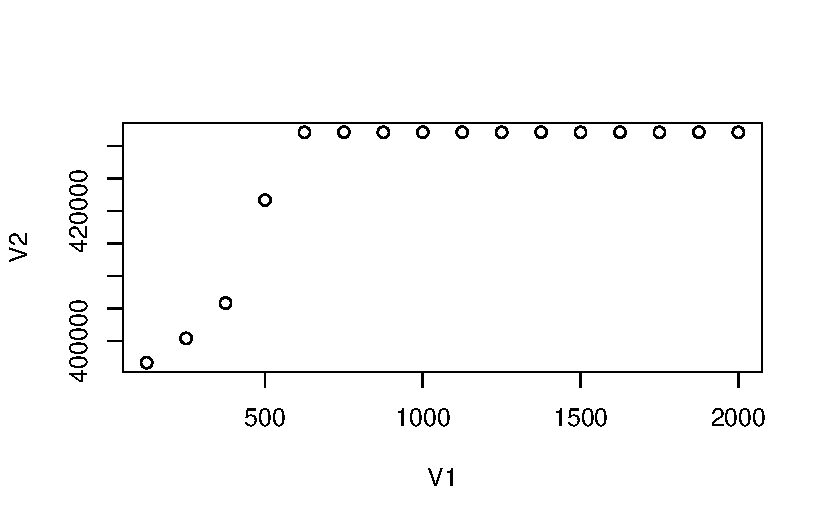
\includegraphics{geo-hw-spdep_files/figure-pdf/unnamed-chunk-17-1.pdf}

}

\end{figure}



\end{document}
